\documentclass[addpoints]{exam}

\printanswers
\CorrectChoiceEmphasis{\color{red}\bfseries}
\usepackage{amssymb, amsmath, amsfonts}
\usepackage{geometry}
\usepackage{graphicx}
\usepackage{tikz}
\usetikzlibrary{calc}
\usepackage{pgfplots}
\usepackage{multirow,array} % for payoff matrix formatting
\usepackage[colorlinks,pdfusetitle,urlcolor=blue,citecolor=blue,linkcolor=blue]{hyperref}
\usepackage{bbding} % dingbats fonts

\usepackage{adjustbox}

\definecolor{crimson}{RGB}{ 170, 4, 36 }
\definecolor{darkblue}{RGB}{ 4, 47, 170 }
\definecolor{brown}{RGB}{ 111, 71, 2 }
\definecolor{periwinkle}{RGB}{ 90, 177, 204 }
\definecolor{ducksgreen}{HTML}{007030}

\geometry{left=1.0in,right=1.0in,top=1.0in,bottom=1.0in}
\pagestyle{headandfoot}
\lhead{EC327 Game Theory}
\chead{Homework 5}
\rhead{Fall 2025}
\runningheadrule

\title{
    \textbf{Econ 327: Game Theory} \\ 
    Homework $\#8$
    }
\author{University of Oregon}
\date{Due: Dec. 5$^{th}$}

% exam-type question formatting
\renewcommand{\thequestion}{\textbf{Q\arabic{question}}}
\bracketedpoints

\begin{document}

\maketitle

\begin{center}
  \gradetable[h][questions]
\end{center}

\vspace{0.5in}

\begin{center}
  \textbf{For homework assignments:}
\end{center}

\begin{itemize}

%  \item DO NOT write your name:
%  this assignment will be graded anonymously. 
%  If you want to, you can include your student ID instead.

  \item Complete \textit{all} questions and parts.

  % I will select one question at random to be graded
  % according to the rubric on Canvas.

  \item You will be graded on not only the content of your work
    but on how clearly you present your ideas.
    Make sure that your handwriting is legible.
    Please use extra pages if you run out of space 
    but make sure that all parts of a question 
    are in the correct order when you submit.

  \item You may choose to work with others,
  but everyone must submit to Canvas individually.

  Please include the names of everyone who you worked with 
  below your own name.
 
\end{itemize}

\vspace{1.0in}

\makebox[.6\textwidth]{Name\enspace\hrulefill}


\vspace{0.5in}

\begin{center}
  \fbox{\fbox{\parbox{5.5in}{\centering
  \textbf{Note:}
  All Questions are adapted from problems in  
  Dixit, Skeath and Reiley, \textit{Games of Strategy}, Fourth Edition. 
  }}}
\end{center}

\newpage

\begin{questions}
  \question
  Recall the example from the midterm, 
  where South Korea and Japan compete in the market for production of VLCCs. 
  Assume now that the cost of building ships is \$30 (million) in each country, 
  and the demand for ships is $P = 180 - Q$,
  where $Q = q_{\text{Korea}} + q_{\text{Japan}}$.
  \begin{parts}
    \part [4]
    Solve for all Nash equilibria in this continuous strategy game.
    \begin{solution}
      Japan's profit depends on Korea's quantity through the demand curve
      (and vice versa). 
      The profit function (in millions) is Price$\times q - 30q$.
      \begin{align*}
        \Pi_J & = (180 - q_J - q_K)\times q_J - 30\times q_J \\
        \frac{\partial \Pi_J}{\partial q_J} & = 180 - 2q_J - q_K - 30 \\
        BR_J(q_K) & = \frac{150 - q_K}{2}
      \end{align*}
      The game is symmetric, so $BR_K(q_J) = \frac{150 - q_J}{2}$. \\
      In Nash eq, $BR_{J}(q^*_K) = q^*_J$.
      In other words, we can plug in Korea's optimal $q^*_K$ 
      into Japan's best response function:
      \begin{align*}
        q^*_J & = \frac{150 - \left(\frac{150-q^*_J}{2}\right)}
                     {2} \\
      \end{align*}
      Solving for $q^*_J$,
      we get that the intersection of the best responses occurs at:
      $$q^*_J  = 50 = q^*_K$$.
    \begin{center}
    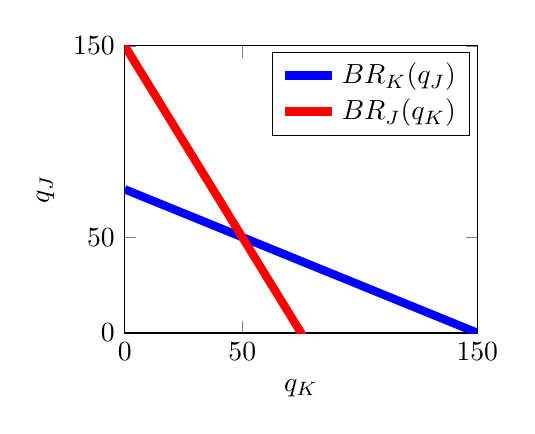
\begin{tikzpicture}
      \begin{axis}[
        width=.5\textwidth,
        xlabel={$q_{K}$},
        ylabel={$q_{J}$},
        xmin=-0.1, xmax=150,
        ymin=-0.1, ymax=150,
        xtick={0,50,150},
        ytick={0,50,150},
        ]
        \addplot [
        domain=0:150,
        line width=3pt,
        color=blue,
        ] 
        {75-0.5*x};
        \addlegendentry{\(BR_K(q_J)\)}
        \addplot [
        domain=0:150,
        line width=3pt,
        color=red,
        ] 
        {150-2*x};
        \addlegendentry{\(BR_J(q_K)\)}
      \end{axis}
    \end{tikzpicture}
    \end{center} 
    \textbf{Nash Eq:} 
    \begin{itemize}
      \item Korea produces $q^*_K = 50$ ships
      \begin{itemize}
        \item Korea's payoff is $\Pi_K = (180 - 50 - 50) \times 50 - 30 \times 50 = 2500$
        \item Or \$2.5 trillion profit
      \end{itemize}
      \item Japan produces $q^*_J = 50$ ships
      \begin{itemize}
        \item Japan's payoff is $\Pi_J = (180 - 50 - 50) \times 50 - 30 \times 50 = 2500$
        \item Or \$2.5 trillion profit
      \end{itemize}
    \end{itemize}
    \end{solution}
    \part [4] 
    Now find the collusive outcome.
    What total quantity should be set by the two countries 
    in order to maximize their joint profit?
    \begin{solution}
      If Japan and Korea are to collude, they should act as a monopolist
      and choose the total output $Q$ to maximize the total profit in the market.
      \begin{align*}
        \Pi_{\text{Total}} & = (180 - Q)Q - 30Q \\
        \frac{\partial \Pi_{\text{Total}}}{\partial Q} & = 180 - 2Q - 30 \\
        Q^* & = \frac{150}{2} = \underline{75}
      \end{align*}
      So if they split the production equally,
      $q_J = q_K = 37.5$ ships each (assuming strategies are continuous). \\
      \textbf{Collusive outcome}:
      \begin{itemize}
        \item Korea produces $q_K^{Col.} = 32.5$ ships
        \begin{itemize}
          \item Korea's payoff is $\Pi_K = (180 - 37.5 - 37.5) \times 37.5 - 30 \times 37.5 = 2,812.5$ 
          \item or about \$2.8 trillion.
        \end{itemize}
        \item Japan produces $q_J^{Col.} = 32.5$ ships
        \begin{itemize}
          \item Japan's payoff is $\Pi_J = (180 - 37.5 - 37.5) \times 37.5 - 30 \times 37.5 = 2,812.5$ 
          \item or about \$2.8 trillion.
        \end{itemize}
      \end{itemize}
    \end{solution}
    \part [4]
    Suppose the two countries produce equal quantities of VLCCs, so
    that they earn equal shares of this collusive profit.
    How much profit would each country earn? 
    Compare this profit with the amount they would earn in the Nash equilibrium.
    \begin{solution}
      See part (b) solution for profit calculations. \\
      By colluding, Japan and Korea could increase both of their profits
      compared to the outcome in part (a).
      Compare the total profit of \$5 trillion in NE
      to the monopolists profit of \$5.625 trillion 
      to see that there are potential gains to collude.
    \end{solution}
    \part [4] 
    Now suppose the two countries are in a repeated relationship.
    Once per year, they choose production quantities,
    and each can observe the amount its rival produced in the previous year. 
    They wish to cooperate to sustain the collusive profit levels found in part (c). 
    In any one year, one of them can defect from the agreement.
    If one of them holds the quantity at the agreed level, 
    what is the best defecting quantity for the other? 
    What are the resulting profits?
    \begin{solution}
      Suppose that Korea keeps their production at the collusive quantity 
      $q_K^{Col.} = 32.5$
      If Japan defects from their collusive quantity,
      to maximize their individual profit
      they should use their best response rule from part (a):
      \begin{align*}
        BR_J(q_K^{Col.} = 32.5) & = \frac{150 - 32.5}{2} = 56.25
      \end{align*}
    \begin{center}
    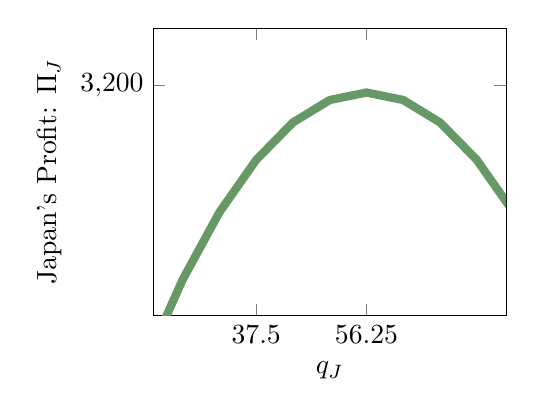
\begin{tikzpicture}
      \begin{axis}[
        width=.5\textwidth,
        xlabel={$q_{J}$},
        ylabel={Japan's Profit: $\Pi_{J}$},
        xmin=20, xmax=80,
        ymin=2000, ymax=3500,
        xtick={0,37.5,56.25},
        ytick={0,3200},
        ]
        \addplot [
        domain=0:150,
        line width=3pt,
        color=green!20!gray,
        ] 
        {(150 - 37.5 - x)*x};
        % \addlegendentry{\(\Pi_J(q_J,q_K = 37.5)\)}
      \end{axis}
    \end{tikzpicture}
    \end{center} 
    The graph above show's that when Japan holds Korea's strategy constant at 37.5,
    their profit function has a single maximum at their best-response strategy of 56.25 ships.
    Producing any more or any less would result in a strictly lower payoff. \\
    \textbf{Unilateral Defection Outcome:}
    \begin{itemize}
      \item Korea produces $q_K^{\text{Col.}} = 37.5$ ships
      \item Japan best responds with $q_J^{\text{Cheat}} = 56.25$ ships
      \begin{itemize}
        \item Korea's payoff is $\Pi_K^{\text{Cheated}} = (180 - 37.5 - 56.25)\cdot 37.5 - 30\cdot37.5 = 2,109.375$
        \item or about \$2.1 trillion
        \item Japan's payoff is $\Pi_J^{\text{Cheat}} = (180 - 37.5 - 56.25)\cdot 56.25 - 30\cdot 56.25 = 3,164.0625$
        \item or about \$3.2 trillion.
      \end{itemize}
    \end{itemize}
    \end{solution}
    \part[4]
    Write down a matrix that represents this game as a prisoners’ dilemma.
    \begin{solution}
      Using the profits for each combination of the individual quantities
      we have used so far yields the following normal form game table
      (where payoffs are in trillions of dollars):
      \begin{center}
        \begin{tabular}{*{5}{c|}}
          \multicolumn{2}{c}{} & \multicolumn{3}{c}{Korea} \\ \cline{3-5}
          \multicolumn{1}{c}{} & & $q_K=37.5$ & $q_K=50$  & $q_K=56.25$\\ \cline{2-5}
          \multirow{3}*{Japan}
          & $q_J=37.5$  & 2.8,~2.8 & 2.4,~3.1 & 2.1,~\underline{3.2} \\ \cline{2-5}
          & $q_J=50$    & 3.1,~2.4 & \underline{2.5},~\underline{2.5} & \underline{2.2},~2.4 \\ \cline{2-5}
          & $q_J=56.25$ & \underline{3.2},~2.1 & 2.4,~\underline{2.2} & 2.1,~2.1 \\ \cline{2-5}
        \end{tabular}
      \end{center}
      We can simplify this into something which looks more like the Prisoners' Dilemma
      by defining the discrete strategies as either produce high ($q=37.5$)
      or produce low ($q=50$ or $q=56.25$ depending on which is BR to opponent).
      \begin{center}
        \begin{tabular}{*{4}{c|}}
          \multicolumn{2}{c}{} & \multicolumn{2}{c}{Korea} \\ \cline{3-4}
          \multicolumn{1}{c}{} & & Low & High  \\ \cline{2-4}
          \multirow{3}*{Japan}
          & Low  & 2.8,~2.8 & 2.1,~\underline{3.2} \\ \cline{2-4}
          & High & \underline{3.2},~2.1& \underline{2.5},~\underline{2.5} \\ \cline{2-4}
        \end{tabular}
      \end{center}
    \end{solution}
    \part[4] 
    For what interest rates will collusion be sustainable 
    when the two countries use grim (defect forever) strategies?
    \begin{solution}
      There are multiple ways that you could define a grim trigger strategy.
      One example is as follows:
      $\begin{cases}
        \text{In } t=1, ~ \text{produce } Low \\
        \text{In } t>1, 
        \begin{cases}
          \text{produce } Low \text{ if opponent has always produced Low before}  \\
          \text{produce } High \text{ if opponent has ever produced High}  \\
        \end{cases}
      \end{cases}$ \\
      Let the the discount factor $\delta = \frac{1}{1+r}$  
      be the subjective discount factor 
      determined by the interest rate $r$. \\
      To generalize the Prisoners' Dilemma payoffs,
      lets represent the payoff to both countries of cooperating as $V_C$,
      $V_D$ as the payoff from defecting against an opponent who set a Low production,
      and $V_N$ as the payoff in the Nash equilibrium of mutual High production. \\
      Then either country will continue to choose the Low production
      prescribed by the collusive outcome in part (b)
      when the present value of doing so
      is greater than the present value of ever defecting to a High level of production. \\
      \begin{align*}
        V_C + \frac{\delta V_C}{1-\delta} & \geq V_D + \frac{\delta V_N}{1-\delta} \\
        % V_C - \delta V_C + \delta V_C & \geq V_D - \delta V_D + \delta V_N \\
        \delta (V_D - V_N) & \geq V_D - V_C \\
        \delta & \geq \frac{V_D - V_C}{V_D - V_N}
      \end{align*}
      Using the payoffs from our Prisoner's Dilemma game in part (e),
      this is expressed as the following inequality:
      \begin{align*}
        \delta & \geq \frac{3164.0625 - 2812.5}{3164.0625 - 2500} \\
        \delta & \geq 0.53
      \end{align*}
      If you choose to express this in terms of the interest rate $r$:
      \begin{align*}
        \frac{1}{1+r} & = 0.53 \\
        % 1 & = 0.53 + 0.53r \\
        r & \leq 0.89 \\
      \end{align*}
    \end{solution}
  \end{parts}

  \newpage 

  \question
  Glassworks and Clearsmooth compete in the local market for windshield repairs.
  The market size (total available profits) is \$10 million per year.
  Each firm can choose whether to advertise on local television. 
  If a firm chooses to advertise in a given year, 
  it costs that firm \$3 million.
  If one firm advertises and the other doesn’t, 
  then the former captures the whole market.
  If both firms advertise, they split the market 50:50.
  If both firms choose not to advertise, they also split the market 50:50.

  \begin{parts}
    \part[4]
    Suppose the two windshield-repair firms know they will compete for just one year.
    Write down the payoff matrix for this game.
    Find the Nash equilibrium strategies.
    \begin{solution}
      \begin{center}
        \begin{tabular}{*{4}{c|}}
          \multicolumn{2}{c}{} & \multicolumn{2}{c}{Glassworks} \\ \cline{3-4}
          \multicolumn{1}{c}{} &                & Advertise & Don't  \\ \cline{2-4}
          \multirow{3}*{Clearsooth} & Advertise & 2, 2      & 7, 0\\ \cline{2-4}
                                    & Don't     & 0, 7      & 5, 5 \\ \cline{2-4}
        \end{tabular}
      \end{center}
      \textbf{Nash Eq:} Both frims Advertise, 
      because this strategy dominates Don't for both.
    \end{solution}
    \part[4]
    Suppose the firms play this game for five years in a row, 
    and they know that at the end of five years,
    both firms plan to go out of business.
    What is the subgame-perfect equilibrium for this five-period game? 
    Explain. 
    \begin{solution}
      At year 5, both should anticipate that the only rational choice is to Advertise
      because this is the dominant strategy in that subgame.
      Using backwards induction, the best response in any period
      from the first year onward is also to Advertise each period. \\
      \textbf{SPNE:} Both firms Advertise every year.
    \end{solution}
    \part[4]
    What would be a tit-for-tat strategy in the game described in part (b)?
    \begin{solution}
      There are multiple ways to define a tit-for-tat strategy for this game.
      But any version should start out with not advertising
      to try to get the competing firm to also not advertise.
      There should be some punishment if the other firm does Advertise. \\
      \textbf{Tit-for-tat strategy:}
      \begin{itemize}
        \item In year 1: \texttt{Don't} advertise
        \item In all years after year 1:
        $\begin{cases}
          \texttt{Don't}\text{ if other firm \textit{never} advertised} \\
          \texttt{Advertise} \text{ if other firm \textit{ever} advertised}
        \end{cases}$
      \end{itemize}
    \end{solution}
    \part[4]
    Suppose the firms play this game repeatedly forever, 
    and suppose that future profits are discounted
    with an interest rate of 20\% per year.
    Can you find a subgame-perfect equilibrium that involves higher annual payoffs than the equilibrium in part (b)?
    If so, explain what strategies are involved.
    If not, explain why not.
    \begin{solution}
      While the tit-for-tat strategy wouldn't work to sustain cooperation
      in the repeated game with a certain finite number of years in part (b),
      when the game is \textit{infinitely} repeated, 
      the Folk Theorem tells us cooperation may be sustained for
      some individually rational strategy profile
      with sufficiently patient players. \\
      Let's use the tit-for-tat strategy defined in part (c)
      to test what level of discounting is necessary. \\
      If either country is going to defect against a tit-for-tat player,
      they should do so in the first period to get the immediate benefit of 7.
      It is still possible that they can go back to the cooperative annual profit of 5
      as long as they take the lower payoff of 0 for the period after defection.
      \begin{itemize}
        \item present value of defecting once: $7 + 0\delta + 5\delta^2 + 5\delta^3 + \dots$
        \item present value of cooperating forever: $5 + 5\delta + 5\delta^2 + 5\delta^3 + \dots$
      \end{itemize}
      So cooperation is sustainable as long as both firms are patient enough
      (high enough discount factor)
      such that there is never an incentive to cheat:
      \begin{align*}
        5 + 5\delta + \frac{5\delta^2}{1-\delta} & \geq 7 + 0 + \frac{5\delta^2}{1-\delta} \\
        5 + 5 \delta & \geq 7 \\
        \delta & \geq 2/7 \\
      \end{align*}
      If we plug in the interest rate of 20\% into $\frac{1}{1+r}$,
      then we get that the discount rate of these firms is
      $1/1.2 = 0.83$.
      So this is patient enough that tit-for-tat can sustain repeated cooperation.
    \end{solution}
  \end{parts}
  
\end{questions}
\end{document}